% ----------------------------------------------------------------
% Revisão bibliográfica *******************
% ----------------------------------------------------------------
\chapter{Desenvolvimento}
\label{cap:desenvolvimento}
%
%
O desenvolvimento da \textit{SAGA Game Library} ou SGL, assim como todo \textit{software}, passou por diversas etapas, para que no final fosse possível obter um produto condizente com a proposta do trabalho.
\par 
O desenvolvimento de um \textit{software}, de maneira geral, sempre é composto das seguintes etapas:
%
\begin{itemize}
\item Especificação dos requisitos do \textit{software}: Descrição do objetivo e do que se espera do \textit{software}.
\item Projeto do sistema: decisão dos conceitos relacionado ao que deve ser implementado, incluindo a escolha da linguagem de programação adequada, sistema operacional alvo, bibliotecas e ferramentas auxiliares.
\item Implementação: O próprio desenvolvimento do \textit{software}. Consiste na transformação de todo o conteúdo formulado na fase de projeto em código.
\item Teste e depuração: Fase que consiste no teste do \textit{software} já implementado e na procura e correção de erros.
\end{itemize}
%
\par 
A SGL também seguiu de maneira consistente as etapas acima. A seguir serão descritas as particularidades de cada uma delas.
%
%
%
%
% ----------------------------------------------------------------
% Especificao requisitos *******************
% ----------------------------------------------------------------
\section{Especificação dos requisitos do projeto}
%
O objetivo inicial deste trabalho de conclusão de curso consistia na implementação de um \textit{game online} que utilizasse toda a base teórica vista durante o curso de graduação. Entretanto após analise do conteúdo e recursos necessários para realizar tal projeto, concluiu-se que o mesmo demandaria um custo alto, tanto em relação a mão-de-obra quanto ao conhecimento necessário para fazê-lo. Com base nessa conclusão, seguimos em busca de outros temas de projeto ainda relacionados a área de jogos eletrônicos. Após alguns estudos sobre o mercado de desenvolvimento de jogos, chegamos ao consenso de desenvolver uma biblioteca de desenvolvimento de jogos voltada para o meio acadêmico.
\par 
A escolha do público alvo da biblioteca teve grande influência nos requisitos exigidos no desenvolvimento desse \textit{software}. Uma vez que a biblioteca deveria ser voltada ao meio acadêmico, ou seja, ao ensino, ela deveria apresentar uma baixa curva de aprendizado, sem dispensar recursos importantes para uma \textit{game engine}. A seguir, estão listados os requisitos que a biblioteca deverá apresentar ao final de sua implementação.
%
\subsection{Baixa curva de aprendizado}
%
Como dito anteriormente, a biblioteca é voltada para estudantes e entusiastas que possuem pouca ou mesmo nenhuma experiência na área de programação de jogos eletrônicos. Assim, torna-se essencial que a \textit{engine} seja de fácil uso, de modo que o usuário sinta-se a vontade e amparado para desenvolver seus projetos e não desestimulado por utilizar uma ferramenta que apresenta uma complexidade muito grande no uso.
%
\subsection{Gerenciamento automático de recursos}
%
No desenvolvimento de jogos, os chamados recursos ou \textit{resources}, são arquivos de imagens, fontes de texto \textit{True Type} e arquivos de áudio. O gerenciamento de recursos proporciona uma considerável redução no uso da memória RAM destinada aos recursos e no tempo de carregamento dos mesmos.
%
\subsection{Arquitetura multi-plataforma}
%
Um dos requisitos fundamentais da biblioteca. Um dos principais objetivos da SGL é ser compatível com o maior números de plataformas possíveis, de modo que o usuário sinta-se a vontade para desenvolver em sua plataforma preferida.
%
\subsection{Suporte a diversos formatos de arquivos}
%
Suporte a arquivos de imagens (.PNG, .JPG e .BMP), fontes \textit{True Type} e reprodução de arquivos de áudio (.ogg e .wav). São os tipos de arquivos mais comuns utilizados nos jogos. As fontes \textit{True Type} são preferidas ao invés da fontes \textit{bitmap}, por estas últimas não suportarem \textit{anti-alising}. 
%
\subsection{Renderização acelerada por \textit{hardware} e gráficos 2D}
%
Um pré-requisito para todas \textit{game engines} é fazer uso dos \textit{hardwares} mais atuais. Algumas APIs, como a popular SDL, possuem suporte apenas à renderização por software para gráficos 2D, o que aumentava consideravelmente o uso do processador durante as rotinas de desenho do jogo. O único modo de obter a aceleração por \textit{hardware}, usando diretamente a placa de vídeo, era utilizar a OpenGL para realizar as rotinas de renderização. Esse hibridismo entre SDL e OpenGL aumenta em muito a complexidade de implementação de um jogo, onde a aceleração por \textit{hardware} se faz necessária. Com isso em mente, a \textit{SAGA Game Library} deveria fornecer essa aceleração por \textit{hardware} para rotinas de renderização 2D, de modo que o desenvolvedor que estivesse utilizando a biblioteca não precisasse se preocupar em usar outras APIs para esse fim.
%
\subsection{Suporte a eventos de sistemas e a dispositivos de entrada}
%
A biblioteca deveria ser capaz de receber eventos de teclado, \textit{mouse} e \textit{joystick}. Suporte a dispositivos com tela \textit{tounch} era uma opção secundária.
%
\subsection{Suporte ao editor de níveis Tiled}
%
A edição de níveis ou cenários é uma das tarefas mais complexas no desenvolvimento de um jogo. Todo o processo, desde a elaboração artística do cenário até a maneira como o jogador irá interagir com o mesmo, exige muito planejamento e demanda muito esforço em sua implementação. Com o objetivo de facilitar esse trabalho, surgiram os editores de níveis. 
\par
Os editores de níveis são \textit{softwares} destinados à construção de cenários em jogos, o que faz deles ferramentas de grande importância para uma \textit{game engine}. Neste ponto, existem duas opções disponíveis para quem deseja implementar uma \textit{engine}: desenvolver seu próprio editor ou utilizar um editor externo, desenvolvido por terceiros. Desenvolver um editor próprio demanda muito estudo e tempo de desenvolvimento, além do que já é necessário para implementar a \textit{engine}. Tendo isso em mente, chegou-se à conclusão de que o melhor seria oferecer suporte a um editor externo, no que o editor Tiled foi escolhido. 
\par
O software Tiled \cite{SiteTiled} é uma ferramenta gratuita desenvolvida em C++ para a criação de \textit{layouts} e mapas usando \textit{tilesets}, baseado na técnica de \textit{Tilemap}. Ele suporta mapas com projeções ortogonais e isométricas e ainda permite que objetos personalizados sejam salvos como imagens na resolução que se desejar. Tem suporte também a comandos externos, \textit{plugins} e formatos usados por outros editores. É possível, ainda, redimensionar e alterar o mapa posteriormente, criar múltiplos mapas em uma única sessão e ainda salvar ou restaurar até nove vezes. Com ele pode-se especificar o tamanho de cada \textit{tile} em um \textit{tileset}, ou criar um mapa sem tamanho estrito sobre as imagens \cite{TiledTutorial}.
%
\begin{figure}[H]
    \centering
		\caption{\textit{printscreen} da interface do Tiled.}
    \label{tiledGUI}
    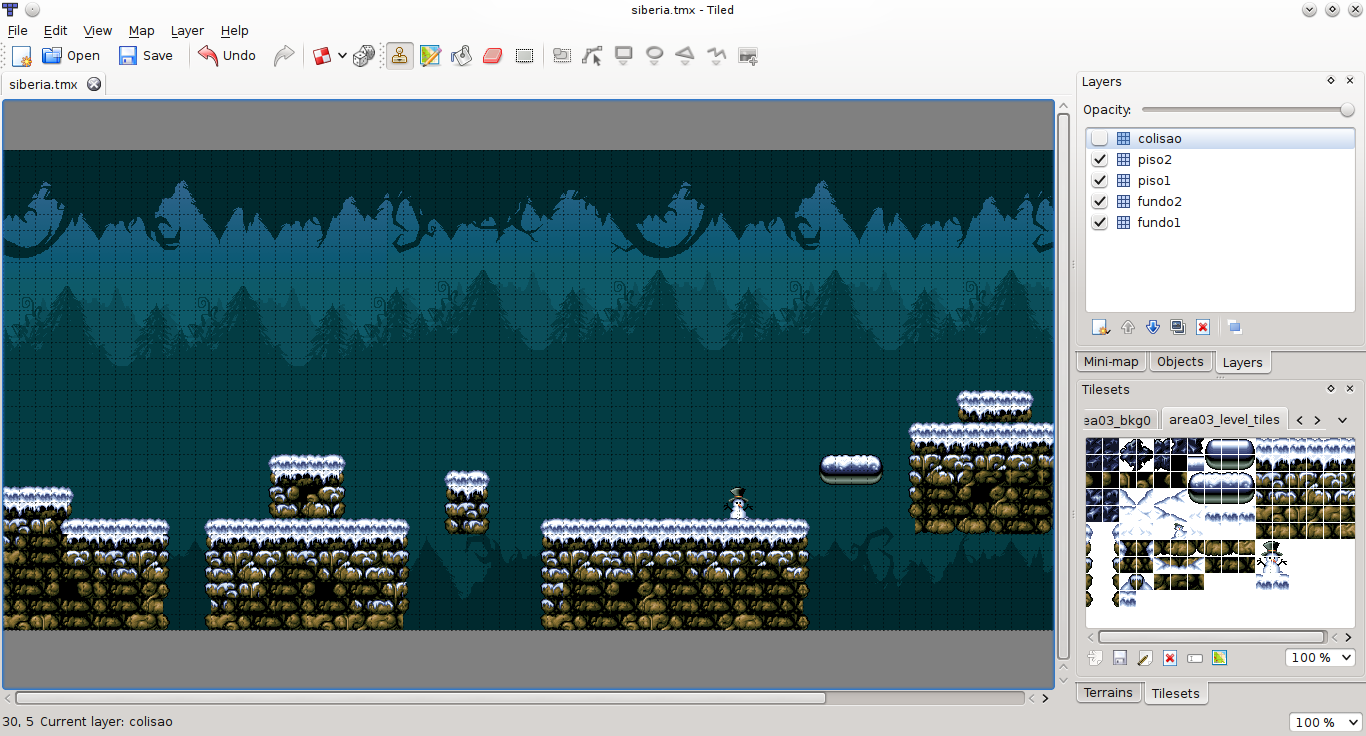
\includegraphics[scale = 0.45]{Imagens/Tiled.png}
\end{figure}
%
\par
Mesmo que o desenvolvedor não queira que seu jogo seja baseado em \textit{tiles}, o software é ainda uma excelente escolha como um editor de níveis. Pode-se usá-lo também nas entidades invisíveis, tais como áreas de colisão e o aparecimento de objetos dentro do 
mapa. Por sua simplicidade ela pode ser usada por programadores iniciantes ou experientes.
%
%
%
%
% ----------------------------------------------------------------
% Projeto do sistema *******************
% ----------------------------------------------------------------
\section{Projeto do sistema}
%
Uma vez definidos os requisitos do sistema, a próxima etapa era dar início ao desenvolvimento do projeto. O primeiro passo foi definir, com base nos requisitos e no conhecimento dos envolvidos, qual seria a linguagem de programação mais adequada ao problema e qual API deveríamos usar para as rotinas de renderização, leitura dos dispositivos de entrada, reprodução de áudio, etc.
%
%
\subsection{Linguagem de Programação}
\label{linguagem}
%
Até a década de 90 cada jogo tinha a sua \textit{engine}, feita para possibilitar a maior eficiência no uso da memória e da unidade de processamento possível, de acordo com as exigências de cada jogo. Um jogo que só usava formas geométricas, por exemplo, não precisava tratar imagens na sua \textit{engine}. O nível da microeletrônica e da computação já possibilita o uso de \textit{engines} genéricas, mas o desenvolvimento de uma ainda demanda uma programação muito próxima da máquina. 
\par
É por isso que a escolha da linguagem de programação precisa ser feita com cuidado. Considerando o conhecimento da equipe e o propósito do projeto, que era uma \textit{engine} didática, para influenciar o \textit{designe} e o desenvolvimento de jogos de acordo com o nosso alcance, as linguagens de programação selecionadas para a análise foram Actionscript, C++, C\# e Java, de acordo com a simplicidade, o poder e a compatibilidade de cada uma.
%
\subsubsection{Estudo Comparativo}
%
O Actionscript é uma linguagem orientada a objetos desenvolvida pela Macromedia. O que no início era uma ferramenta para controlar animações se tornou uma linguagem de script tão complexa que podia ser usada no desenvolvimento de um jogo. Embora essa linguagem ainda seja muito usada no desenvolvimento de jogos de web, o que provocou a decisão contrária a ela foi a expectativa de que o HTML 5 viesse a incorporar o Javascript e, dessa forma, modificar ou inutilizar o Actionscript.
\par
O C\# (C Sharp) é uma linguagem multi-paradigma da Microsoft feita para o desenvolvimento de sistemas próprios para a plataforma .NET. C\# e Java compartilham a mesma simplicidade na leitura e na codificação, assim como a mesma forma de interpretação e compilação, mas um programa em C\# está mais próximo da máquina do que um programa em Java. A escolha parecia feita quando nós entendemos que a ligação do C\# com a Microsoft poderia custar a compatibilidade do nosso jogo.
\par
Java é uma linguagem orientada a objetos desenvolvida pela Sun, hoje possuída pela Oracle. A sua fama de espaçosa e pesada não é coerente com a realidade: hoje a linguagem conta com a Compilação na Hora ou \textit{Just in Time Compilation} (\textit{JIT Compilation} ou só JIT), para que a sua execução não seja mais interpretada. Mas a sua principal característica é a compatibilidade: a Máquina Virtual do Java ou Java Virtual Machine (JVM) é uma plataforma virtual que pode ser feita compatível para qualquer plataforma física.
\par
Por mais evoluída que seja a JVM, no entanto, o Java não admite o acesso à máquina necessário para o desenvolvimento de uma \textit{game engine}, senão com o uso do C++, por meio da Interface Nativa do Java ou Java Native Interface (JNI). Em outras palavras, para usar o Java, nesse caso, nós teríamos que usar o C++. Esta, por sua vez, não é a mais simples na codificação, mas não tem limitação alguma tanto em termos de 
compatibilidade quanto em termos de acesso à máquina.
%
\subsubsection{A Escolha: C++}
%
C++ (C Mais Mais ou C Plus Plus) \cite{Mizrahi} é uma linguagem de programação multi-paradigma, com suporte para a programação imperativa e a programação orientada a objetos, de uso geral, desenvolvida por Bjarne Stroustrup, para formar uma camada de orientação a objetos sobre a linguagem de programação C. O C++ possibilita a programação de baixo nível assim como a programação de alto nível e por isso é considerado uma linguagem de programação de nível médio em termos de proximidade da máquina.
\par
Após o estudo comparativo acima, concluímos que a linguagem C++ seria a melhor opção para o projeto em questão. Tal decisão foi baseada em diversos fatores, como experiência e domínio da linguagem pelos envolvidos no projeto, o desempenho das aplicações escritas nesta linguagem e o fato de C++ ser a linguagem de programação mais usada no desenvolvimento de jogos. Uma vez que o objetivo da biblioteca é ser uma porta de entrada para essa área, a escolha da linguagem faz com que o usuário já se familiarize com a mesma. Por último e não menos importante, o C++ é uma linguagem 100\% compatível com a API escolhida como base para a nossa \textit{engine} que será abordada a seguir.
%
%
\subsection{Allegro}
\label{allegro}
%
Nas nossas pesquisas para escolher uma biblioteca com a qual trabalhar, duas se destacaram: a Allegro e a SDL. A SDL (Simple Direct Media Layer -- Camada de Mídia Direta Simples) é uma popular biblioteca multimídia simples de usar, multiplataforma, de código aberto, e amplamente usada para fazer  jogos e aplicações multimídia. Ela também poderia atender às nossas necessidades, mas a Allegro se destacou por ter um código mais limpo e intuitivo, e rotinas específicas para o desenvolvimento de jogos, como renderização acelerada por hardware e suporte nativos a diversos formatos de imagens e arquivos de áudio. Por esta razão ela foi escolhida.
\par 
Allegro \cite{AllegroDoc} é uma biblioteca gráfica multiplataforma, de código fonte aberto e feita na sua maioria em C, mas utilizando internamente também Assembly e C++. Seu nome é um acrônimo recursivo que representa ``\textit{Allegro Low Level Game Routines}'' (``Rotinas de jogo de baixo nível Allegro''). Funciona em diversos compiladores e possui rotinas para a manipulação de funções multimídia de um computador, além de oferecer um ambiente ideal para o desenvolvimento de jogos, tornando-se uma das mais populares ferramentas para esse fim atualmente. Originalmente desenvolvida por Shawn Hargreaves, ela se tornou um projeto colaborativo, com colaboradores de todo o mundo.
\par
Ela possui suporte nativo para rotinas de que utilizam gráficos 2D, embora seja possível utilizá-la em conjuntos com outras APIs, como OpenGL e DirectX, para desenvolvimento de aplicações que utilizem gráficos 3D. Apesar de não ser suficiente para o completo desenvolvimento de um jogo, existem pequenas bibliotecas adicionais (add-ons), feitas para serem acopladas à Allegro, permitindo assim a sua extensão. Através desses add-ons é possível, por exemplo, obter suporte a arquivos MP3, GIF, imagens JPG e vídeos AVI. Isso é útil para que o usuário não tenha que colocar uma porção de funções que não usa na hora de distribuir seu jogo, incluindo somente as partes que for utilizar, diminuindo consideravelmente o tamanho do mesmo.
\par
Atualmente, a biblioteca se encontra na sua quinta versão. Allegro 5 foi completamente reescrita e não apresenta compatibilidade com as suas versões anteriores. Foi feito um esforço para tornar a API mais consistente e segura, o que trouxe melhorias funcionais e uma grande mudança na sua arquitetura, sendo agora orientada a eventos e possuindo suporte nativo a aceleração por hardware. Possui suporte a eventos gerados por dispositivos de entradas como teclado, \textit{mouse} e \textit{joystick} além de funções para desenho de primitivas gráficas, leitura e gravação de seu próprio tipo de arquivo de configuração (muito útil para armazenar configurações e dados de jogos) e é totalmente modular.
\par
A Allegro 5.0 suporta as seguintes plataformas:
%
\begin{itemize}
 \item Windows (MSVC, MinGW);
 \item Unix/Linux;
 \item MacOS X;
 \item iPhone;
 \item Android (Suporte provido pela Allegro 5.1, que ainda se encontra instável).
\end{itemize}
%
A API atualmente se encontra nas versões 5.0.10 (estável) e 5.1.2 (instável). A \textit{SAGA Game Library} foi desenvolvida usando como base a versão 5.0.10, por a mesma ser estável.
\subsubsection{Características Técnicas}

Uma vez que a Allegro é codificada na sua maioria em C, a principal característica dessa biblioteca é a estrutura imperativa. Embora algumas funções internas usem outras técnicas, a interface da Allegro é completamente imperativa, o que determina que a programação de qualquer jogo desenvolvido nessa biblioteca seja imperativa ou híbrida, a não ser que ela própria seja encapsulada.

Outra característica da Allegro profundamente relacionada com a linguagem C é a inexistência de referências. Essa limitação torna a codificação complicada e consequentemente propícia a erros, e a execução ligeiramente mais lenta. Exceto quando a referência não é uma opção (não existem vetores de referências, por exemplo), não há razão para não usá-la. Essa análise é especialmente necessária para o encapsulamento da Allegro.
%
\subsubsection{Principais Recursos e Funções}
%
A seguir, encontramos um conjunto dos principais recursos da Allegro 5, começando com as funções mais gerais da biblioteca.
%
\begin{itemize}
 \item \textbf{al\_init()}: Inicializa a biblioteca Allegro, dando valores a algumas variáveis globais e reservando memória. 
 Deve ser a primeira função a ser chamada.
 \item \textbf{al\_exit()}: Encerra a Allegro. Isto inclui retornar ao modo texto e remover qualquer rotina que tenha sido instalada. 
 Não há necessidade de chamar essa função explicitamente, pois, normalmente, isto é feito quando o programa termina.
\end{itemize}
%
As rotinas de vídeo:
%
\begin{itemize}
 \item \textbf{ALLEGRO\_DISPLAY}: Tipo que representa a janela principal. A biblioteca permite que se trabalhe com múltiplas janelas.
 \item \textbf{al\_create\_display(width, height)}: Cria uma instância da janela, retornando um ponteiro para ALLEGRO\_DISPLAY. 
 Os parâmetros indicam as dimensões em pixels.
 \item \textbf{al\_flip\_display()}: Função para atualizar a tela.
 \item \textbf{al\_destroy\_display(var)}: Finaliza a instância \textit{var} do tipo ALLEGRO\_DISPLAY\*.
\end{itemize}
%
As rotinas para manipulação de arquivos de imagem:
%
\begin{itemize}
 \item \textbf{ALLEGRO\_BITMAP}: Tipo que representa o arquivo de imagem carregado pela Allegro.
 \item \textbf{al\_init\_image\_addon()}: Inicializa o add-on da Allegro 5 para utilização de imagens.
 \item \textbf{al\_load\_bitmap(``example.jpg'')}: Carrega a imagem indicando no parâmetro o nome e tipo. Ela deve estar previamente salva na pasta 
 do programa. Recebe o caminho relativo ou absoluto da imagem a ser carregada, retornando um ponteiro para o tipo ALLEGRO\_BITMAP.
 \item \textbf{al\_draw\_bitmap(bitmap, x, y, mirror)}: Função para desenhar a imagem na tela. Os parâmetros são o bitmap a ser desenhado, as 
 posições x e y e as flags de espelhamento (0, ALLEGRO\_FLIP\_HORIZONTAL, ALLEGRO\_FLIP\_VERTICAL).
\end{itemize}
% 
As rotinas de áudio:
%
\begin{itemize}
 \item \textbf{ALLEGRO\_SAMPLE}: Tipo que representa arquivos pequenos, geralmente efeitos sonoros.
 \item \textbf{ALLEGRO\_AUDIO\_STREAM}: Tipo para representar arquivos grandes, de forma que o arquivo não é carregado de uma vez para a 
 memória. Geralmente representa os arquivos que irão compor uma trilha sonora.
 \item \textbf{al\_install\_audio()} e \textbf{al\_init\_acodec\_addon()}: A primeira inicializa as funções relativas ao áudio. A segunda inicializa os 
 codecs necessários para carregar os diversos formatos de arquivo suportados. Fornece suporte a alguns formatos, como Ogg, Flac e Wave.
 \item \textbf{al\_set\_audio\_stream\_playing(musica, true)}: Função que recebe o arquivo de áudio já carregado no primeiro parâmetro e um tipo 
 booleano no segundo (true para fazê-la tocar ou false, em caso contrário).
 \item \textbf{al\_destroy\_audio\_stream(musica) } e \textbf{al\_destroy\_sample(sample)}: Funções de desalocação dos arquivo de áudio carregados 
 pela Allegro.
\end{itemize}
%
%
A Allegro ainda possui muitos recursos que não foram citados devido a sua quantidade. Posteriormente, a API será explorada mais a fundo conforme os recursos da \textit{SAGA Game Library} forem mostrados.
%
%
\subsection{Suporte ao Tiled}
%
O Tiled faz a edição de várias camadas de \textit{tiles} e salva tudo em um formato padronizado de extensão ``.tmx''. Uma das principais vantagens do formato TMX é sua organização, detalhamento e praticidade, sendo que seu conteúdo pode ser lido através do uso de um \textit{parser} para arquivos XML.
\par 
Existem inúmeros \textit{parsers} de arquivos XML, cada um com suas vantagens e desvantagens. Entre os \textit{parser} mais populares podemos citar a RapidXML e a TinyXML. Segundos comparação do próprio desenvolvedor, a RapidXML apresenta a maior velocidade da leitura de dados entre os \textit{parsers} mais populares, mas o escolhido foi a TinyXML, por sua simplicidade de uso e velocidade que não apresenta uma diferença significativa a sua concorrente RapiXML. 
%
%
\subsubsection{A biblioteca TinyXML}
\label{tinyXML}
%
É uma biblioteca escrita em C++, que analisa uma sequência de entrada no formato XML, permitindo o acesso aos dados contidos nesse último. Em outras palavras, ela realiza o \textit{parser} de uma arquivo .xml e armazena a informação em objetos C++ que podem ser manipulados livremente. 
\par 
A TinyXML \cite{TinyXMLTutorial} pode ser facilmente integrada em outros programas, bastando apenas adicionar seus arquivos ao projeto. Com ela é possível realizar o acesso aos dados direta ou iterativamente, a alteração da estrutura através 
de inserção e remoção de elementos, a remoção de espaços duplicados e a gravação para ficheiros em formato XML.

TinyXML é uma estrutura extremamente compacta e robusta, elaborada para um rápido e fácil aprendizado. Pode ser usada para fins de código aberto ou comerciais. Ela é compatível com UTF-8, de modo a permitir que arquivos XML sejam manipulados em qualquer linguagem humana. Também apresenta grande simplicidade em seu uso e rapidez na leitura de dados.
%
%
\subsubsection{Tiled: Codificação e compactação de dados}
%
%
Um dos recursos mais interessantes do Tiled é a possibilita de exportar os dados contidos no arquivo .tmx de forma compactada e codificação. A principal vantagem do uso dos algoritmos compactação e codificação é a redução do tamanho em disco do arquivo .tmx resultante e o aumento da velocidade de carregamento do cenário, uma vez que a biblioteca carrega os dados codificados e/ou compactados e os decodifica/descompacta a nível de software, ao invés de realizar a leitura dos mesmo em disco. 
\par 
A compactação de dados fornecida pelo Tiled é realizada pelas bibliotecas ZLIB \footnote{ZLIB: http://www.zlib.net/} e GZIP \footnote{GZIP: http://www.gnu.org/software/gzip/gzip.html}, enquanto a codificação é realizada pelo algoritmo Base64 fornecido por \footnote{Algoritmo Base64: http://www.adp-gmbh.ch/cpp/common/base64.html}, também fornecido por uma biblioteca externa. São fornecidas as opções de exportar os dados no arquivo .tmx na forma codificada e compactada ou apenas na forma codificada. Também são oferecidas as opções de exportar os dados em formato puro (sem codificação) XML ou no formato CVS. 
\par 
A seguir podemos verificar a redução do tamanho em disco de um arquivo .tmx em relação ao seu tamanho em disco sem codificação/compactação.
%
\begin{itemize}
 \item Arquivo XML puro( sem codificação/compactação): 31,3 KB;
 \item Com codificação Base64: 9,6 KB;
 \item Com codificação Base64 e compressão GZIP: 2,2 KB;
 \item Com codificação Base64 e compressão ZLIB: 2,1 KB;
 \item No formato CVS: 4,9 KB.
\end{itemize}
%
A \textit{SAGA Game Library} provê suporte total e otimizado às 5 opções de exportação acima. Ela, assim com o Tiled, também faz uso das bibliotecas GZIP e ZLIB para descompactação e também realiza a decodificação dos dados em Base64 contidos no arquivo .tmx (detalhes de uso serão abordados posteriormente).
%
%
%
%
% ----------------------------------------------------------------
% Implementação *******************
% ----------------------------------------------------------------
\section{Implementação da biblioteca}
%
%
A \textit{SAGA Game Library} é uma \textit{engine} orientada a objeto desenvolvida em C++ sobre a API Allegro 5. Ela possui todos os recursos que uma \textit{engine} básica possui, como suporte a criação de \textit{sprites} animados e estáticos, criação de cenários usando o editor de níveis Tiled, suporte ao uso de fontes de texto TTF e a diversos formatos de arquivos de áudio. Também possui gerenciamento de automático de recursos (imagem, fontes e áudio), o que possibilita economia significativa de memória. A biblioteca fornece uma estrutura para implementação do \textit{game loop} e suporte para eventos de teclado, \textit{mouse} e \textit{joystick} também estão presentes. 
\par 
Após a fase de projeto, deu-se sequência à fase de estudo do problema. Esta fase resumiu-se simplesmente no estudo do problema, a fim de torná-lo orientado a objetos. Internamente, a \textit{SAGA Game Library} consiste em um \textit{package} denominado \textit{sgl} e subdivididas em 4 outros \textit{packages} com funções específicas: \textit{image, font, audio e input}.
%
%
\begin{itemize}
 \item image: consiste nas classes exclusivamente relacionadas à parte gráfica da \textit{engine}, o que inclui manipulação de arquivos de imagens como \textit{sprites} animados e estáticos e carregamento e renderização de cenários do jogo;
 \item font: é o responsável pela parte textual da biblioteca. Ele carrega uma fonte no formato TTF (``True Type Font'') padrão do Windows e a utiliza para escrever textos na tela de jogo;
 \item audio: \textit{package} destinado ao carregamento, manuseio e reprodução dos arquivos de áudio;
 \item input: inclui todas as funções relacionadas aos comandos recebidos pelos dispositivos de entradas do computador (teclado, \textit{mouse} e \textit{joystick}).
\end{itemize}
%
Abaixo podemos visualizar o esquema da organização da \textit{engine}. A seguir, serão abordados os principais recursos da biblioteca bem como os detalhes da suas respectivas implementações.
%
%
%
%
\begin{figure}[H]
    \centering
		\caption{Esquema estrutural da SGL. }
    \label{pacotes}
    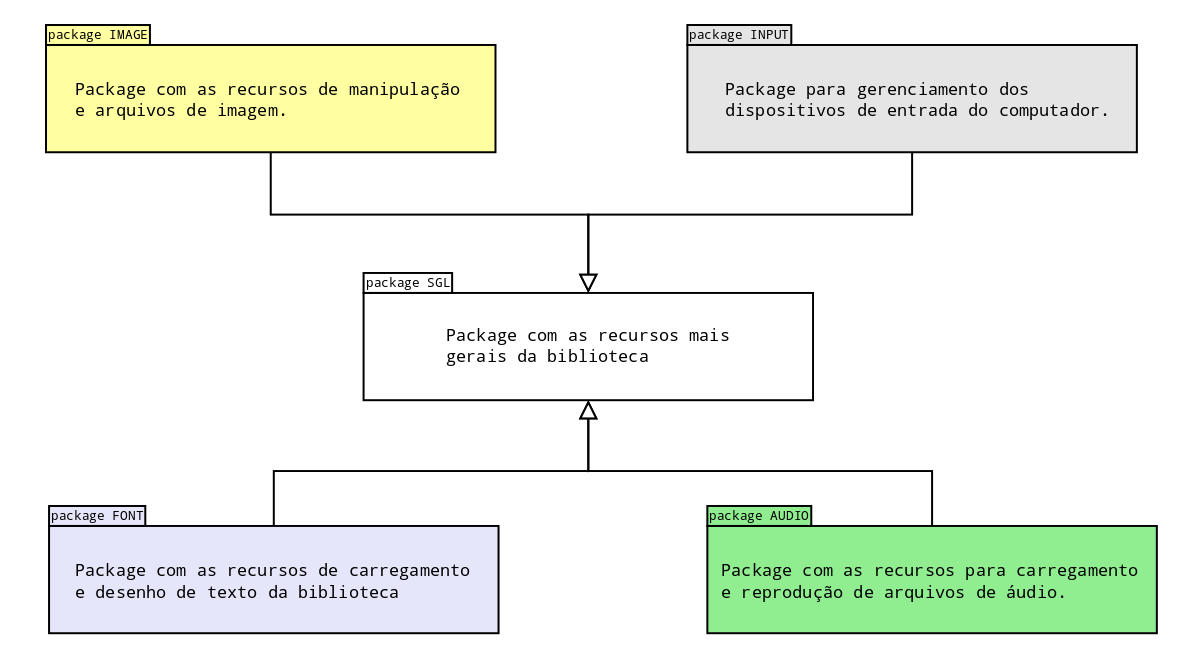
\includegraphics[scale = 0.2]{Imagens/pacotes.png}
\end{figure}
%
%
%
\subsection{SGL}
%
%
É o pacote mais geral, e que engloba todos os outros. Quando a funcionalidade de uma classe não é específica ou é usada como ferramenta auxiliar em outras classes, ela é colocada nesse pacote.
%
%============================================
\subsubsection{AllegroStarter}
%
Cada um dos módulos da Allegro deve ser inicializado antes de seu uso. A Classe AllegroStarter é responsável por alocar e também por desalocar os recursos quando o programa é fechado. Uma exceção é lançada caso algum dispositivo apresente problemas durante a inicialização. Também contém informações sobre a atual versão da Allegro. 
%
%
%============================================
\subsubsection{SGLException}
%
É a classe que captura e trata as exceções que possam ocorrer durante a execução do programa, como inicialização dos componentes da Allegro e carregamento de arquivos de imagem, fonte e áudio. A classe é uma especialização de \texttt{std::exception}. Abaixo temos um exemplo de uso desta classe.
%
\lstinputlisting{CodigoFonte/ExemploSGLException.cpp}
%
\par 
Caso ocorra algum erro de inicialização da Allegro, a função \textit{al\_init()} retornará \textit{false}, fazendo com que o programa execute o conteúdo do \textit{if} e lance a exceção. No console, teremos a mensagem:  ``\textit{terminate called after throwing an instance of `sgl::Exception'
what(): Failed to initialize ALLEGRO\_Lib.}''.
%
%
%============================================
\subsubsection{Color}
%
%
A classe Color possui recursos para trabalharmos com diversos formatos de especificação de cores, como RGB e HTML. Os objetos dessa classe podem ser usadas, por exemplo, para colorir a tela ou alterar a cor de uma determinada fonte de texto. Ela aceita dois construtores. Com o primeiro deles é possível definir cores no formato RGB. Para isso, o construtor recebe três parâmetros que variam de 0 a 255, um para vermelho, outro para verde e outro para azul, respectivamente. O segundo construtor aceita \textit{strings} no formato HTML ou o nome em inglês de uma cor, desde que ele já esteja predefinido. Alguns dos nomes válidos são: \textit{cyan}, \textit{lightgreen}, \textit{green}, entre outros. Caso o nome de uma cor inexistente seja passado como parâmetro, o construtor cria um objeto com as coordenadas RGB iguais a 0 (cor preta). A seguir temos alguns exemplos de uso da classe Color.
%
%
\lstinputlisting{CodigoFonte/ExemploColor.cpp}
%
%
%============================================
\subsubsection{Video}
%
%
Classe responsável por gerenciar todos os recursos de vídeo da \textit{engine}. Através dela, tem-se acesso a todas as rotinas pertinentes (de atualização de tela, posicionamento, e outros eventos) para o gerenciamento de vídeo. A classe também possibilita a escolha por parte do usuário de criar um \textit{display} no formato de janela ou em \textit{fullscreen}, e também permite a escolha de uma API para renderização 3D, como OpenGL (Linux e Windows) e DirectX (Windows). 
\par 
Quando criarmos um objeto da classe Video, devemos definir as dimensões do \textit{display}, passando como parâmetro a largura e altura desejadas e o modo (WINDOWED, FULLSCREEN) no construtor da classe. Por padrão, a cor de fundo do vídeo é preta, podendo ser alterada. Também existe a possibilidade de adicionar um ícone e um título para nossa janela. A função \textit{refresh()} é responsável por por transferir o conteúdo da memória de vídeo para o \textit{display} e deve ser chamada sempre que seja necessário atualizar o \textit{display}, caso contrário, nenhum das ações realizadas pelas rotinas de desenho serão visualizadas. 
\par 
A principal dificuldade na implementação dessa classe foi aprender como a Allegro fazia uso da memória de vídeo e dos conceitos envolvidos, como taxa de atualização do \textit{display}, uso do \textit{vsync} e de como poderíamos tirar o máximo proveito disso. O principal fator foi quanto ao desempenho da renderização da tela. Isso foi resolvido ajustando a Allegro para que a mesma armazenasse todas as imagens a serem desenhadas na memória de vídeo ao invés da memória RAM. Essa configuração apresentou resultados significativos no uso do processador. Enquanto as imagens armazenadas na RAM utilizavam 25\% da CPU, as mesmas imagens armazenadas na memória de vídeo não consumiam mais de 2\% do processador durante o processo de desenho no \textit{display}.
\par
A seguir temos a classe Video em detalhes.
%
%
%
%
\begin{figure}[H]
    \centering
		\caption{UML da classe Video.}
    \label{umlVideo}
    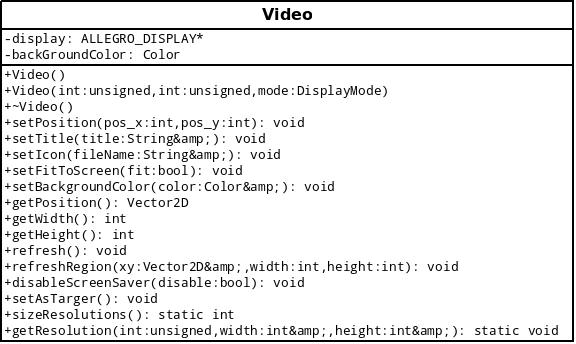
\includegraphics[scale = 0.5]{uml/video.jpeg}
\end{figure}
%
%
E um exemplo de uso da mesma.
%
%
\lstinputlisting{CodigoFonte/ExemploDisplay.cpp}
%
%
\begin{figure}[H]
    \centering
		\caption{Display criado com o uso da classe Video.}
    \label{display}
    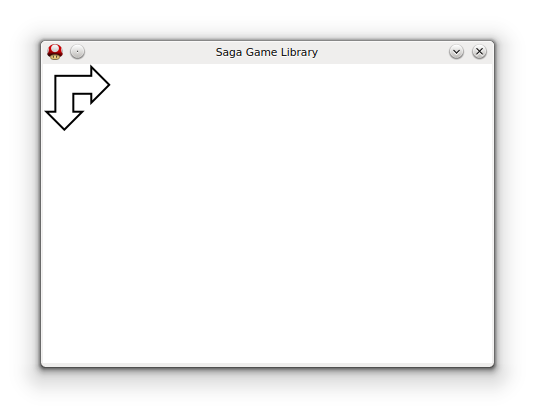
\includegraphics[scale = 0.40]{Imagens/display.png}
\end{figure}
%
%
%============================================
\subsubsection{Vector2D}
%
%
A classe Vector2D é uma das classe mais importantes da \textit{SAGA Game LIbrary}. A classe Vector2D, tal qual o nome diz, define um vetor bidimensional, iniciando-se no ponto (0,0) da tela e indo até o ponto (x,y) definido pelo usuário, sendo responsável pelo posicionamento de qualquer entidade, seja ela um \textit{sprite} ou um texto, no \textit{display}. A escolha do uso de vetores ao invés de simples coordenadas deve-se a vantagens como simplicidade e padronização. Muitas operações matemáticas, como deslocamento, rotações e escalonamentos, são feitas utilizando vetores. Até mesmo efeitos de física, como gravidade e aceleração, são executados usando como base os conceitos da mecânica clássica. A vantagem do vetor sobre um par de coordenadas (x,y) deve-se à quantidade de informação que o primeiro carrega. Enquanto um ponto representa apenas uma localização no espaço, um vetor possui uma direção, sentido e magnitude. 
\par 
Assim como ocorre na geometria, os vetores também possibilitam diversas operações algébricas entre eles, através da sobrecarga de operadores. Soma e subtração de vetores e normalização são algumas das operações possíveis e que podem ser usadas para se obter interessantes resultados, como uma simulação de gravidade, ilustrada na figura abaixo, onde temos um vetor representando o deslocamento do personagem e outro representando a força gravitacional.
%
%
%
\begin{figure}[H]
    \centering
		\caption{Uso de vetores na simulação de gravidade. Fonte: \cite{PontoV}}
    \label{VetorGravidade}
    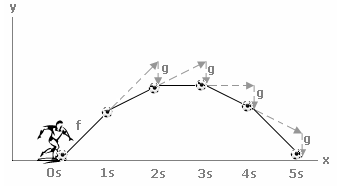
\includegraphics[scale = 0.8]{Imagens/VetorGravidade.png}
\end{figure}
%
%
A seguir temos um exemplo com algumas das operações de Vector2D.
%
\lstinputlisting{CodigoFonte/ExemploVector2D.cpp}
%
%
%============================================
\subsubsection{BoundingBox}
%
%
Esta classe cria um retângulo usando dois objetos Vector2D. Ela possui rotinas para alterar a posição do retângulo e movê-lo e também verifica se há colisão com outro retângulo. É utilizada na biblioteca como um mecanismo para detectar se ocorreu colisão entre duas entidades, como por exemplo, um personagem e um objeto do cenário, como uma parede. Se ocorreu a colisão, o método responsável pela verificação retorna \textit{true}, caso contrário ele retorna \textit{false}. Vale ressaltar que a classe é responsável apenas por verificar se ocorreu ou não colisão, sendo de responsabilidade de quem está desenvolvendo o jogo realizar o tratamento adequado dessa colisão.
%
%
%============================================
\subsubsection{Geometrics}
%
%
Classe usada para desenhar primitivas geométricas. Possui como atributos um inteiro para armazenar a espessura da linha e duas variáveis da classe Color, uma para cor da linha e outra para cor do preenchimento. O construtor padrão inicializa a espessura com 1, a cor de preenchimento como branca e a cor da linha como preta. Outro construtor da ao usuário a liberdade de definir os valores como quiser. Com ela é possível desenhar linhas, triângulos, retângulos, retângulos com cantor arredondados, elipses, círculos e arcos. 
\par 
Exemplos: 
\par
Declaração de vetores que serão usados:
%
\begin{lstlisting}
  Vector2D a(200,150);
  Vector2D b(280,150);
  Vector2D c(350,150);
  Vector2D d(200,100);
\end{lstlisting}
%
%
\par 
No construtor da classe, dizemos que a espessura da linha é 5 e que sua cor é verde. O terceiro parâmetro diz respeito à cor de preenchimento da forma geométrica a ser desenhada. 
%
\begin{lstlisting}
 Geometrics geo(5, Color("green"), Color("purple"));
\end{lstlisting}
%
Em \textit{drawCircle()}, o primeiro parâmetro deve ser a posição do círculo. O segundo é o raio e o terceiro é do tipo booleano. Se for \textit{true}, o objeto será preenchido com a cor definida no construtor. Se for \textit{false}, a forma não terá preenchimento algum. Note que parte do círculo não aparece porque está atrás do triângulo. Se o triângulo não tivesse cor de preenchimento, essa parte iria aparecer. 
%
\begin{lstlisting}
 geo.drawCircle(a, 100, false);
 geo.drawTriangle(b, c, d, true);
\end{lstlisting}
%
%
%
\begin{figure}[H]
    \centering
		\caption{Exemplo de udo da classe Geometrics.}
    \label{ExemploGeometric}
    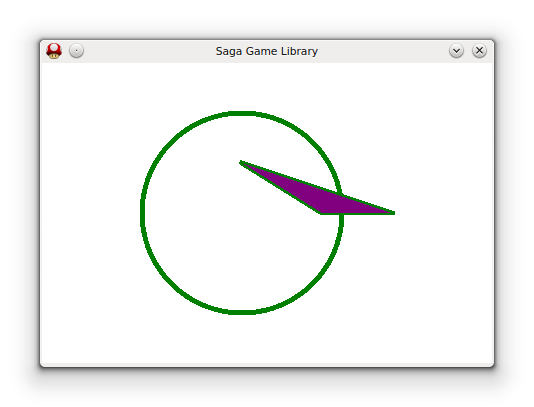
\includegraphics[scale = 0.7]{Imagens/ExemploGeometric.png}
\end{figure}
%
%
%===========================================
\subsubsection{TimeHandler}
%
%
Classe que possui rotinas relacionadas à contagem de tempo. A contagem de tempo é algo muito importante no desenvolvimento de \textit{games}, pois ela pode ser usada para controlar a contagem de atualizações por segundo do \textit{display} ou até mesmo executar ações do jogo que são dependentes do tempo. Através da TimeHandler podemos iniciar, parar, pausar e retornar a uma contagem de tempo. 

O trecho a seguir faz a contagem de tempo necessária para o computador percorrer a extensão de um tipo \textit{unsigned int} em arquitetura 32 bits.
%
\begin{lstlisting}
  TimeHandler time;
  time.start();
  for (unsigned int i = 0; i<4294967295; i++){} 
  time.pause();
  float t = time.getTicks();
\end{lstlisting}
%
\par 
A execução do código acima nos devolve a seguinte saída (em segundos): 
%
\begin{lstlisting}
  t = 17.0142
\end{lstlisting}
%
%===========================================
\subsubsection{Resource e ResourceManager}
%
A classe Resource representa um recurso (áudio, imagem ou fonte) a ser utilizada no jogo e é uma classe abstrata que serve de base para as classes ImageResource, usada para o carregamento de imagens, FontResource utilizada no carregamento de fontes \textit{True Type}, AudioStreamResource e AudioSampleResource, que representam \textit{samples} e \textit{streams} de áudio. Quando um arquivo é carregado, seja ele fonte \textit{True Type}, imagem ou áudio, o mesmo é armazenado em sua respectiva classe filha de Resource. Deste modo conseguimos separar de maneira bem clara cada tipo de recurso, sendo que cada classe filha possui métodos para alocação e desalocação desse recursos pela Allegro além de métodos próprios para se trabalhar com o seu tipo de recurso. 
%
\par
Arquivos como imagens e áudio, podem ocupar tamanho razoável na memória (RAM e ROM) e apresentar um custo computacional considerável quando são carregados. Um jogo eletrônico é um tipo de \textit{software} que sempre busca o máximo em economia de memória e desempenho, isso faz com que o carregamento de uma mesmo recurso várias vezes não seja uma opção. A classe ResourceManager foi criada para corrigir esse inconveniente.
%
%
\begin{figure}[h]
    \centering
		\caption{UML detalhando as classes Resource e ResourceManager.}
    \label{ResourceManager}
    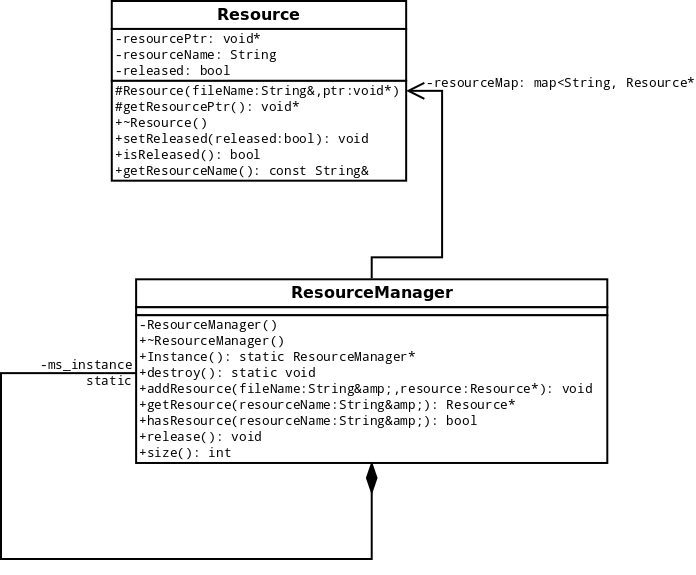
\includegraphics[scale = 0.4]{uml/ResourceManager.png}
\end{figure}
%
%
\par 
A ResourceManager é a classe responsável por executar esse gerenciamento de recursos. Ela possui como principal atributo um objeto da classe \textit{map} da biblioteca STL, chamado \textit{resourceMap}, que usa como chave para armazenamento os \textit{paths} dos recursos carregados.

Esta estrutura permite o gerenciamento dos recursos de forma otimizada, fazendo que haja economia de memória e processamento. É muito mais rápido para o programa apenas reproduzir um recurso já carregado do que ter de carregá-lo novamente. É muito importante ter esse tipo de gerenciamento, especialmente para jogos com imagens muito repetitivas. O algoritmo usado pelas classes que fazem uso do ResourceManager é o seguinte: procuramos pelo objeto (pertencente a uma das classes filhas de Resource), utilizando o nome do seu arquivo, no mapa de Resources na ResourceManager. Se encontrarmos o objeto procurado, a ResourceManager retorna um ponteiro desse objeto, caso contrário criamos esse novo Resource e o inserimos no mapa de Resources. Abaixo podemos verificar o uso desse algoritmo no método que faz o carregamento das imagens na biblioteca. O padrão \textit{Singleton} foi utilizado devido a classe exercer uma papel de gerenciamento, ou seja, ter mais de uma classe gerenciando os recursos criados apenas tornaria mais custosa a utilização da mesma, uma vez que teríamos de procurar do resourceMap de cada ResourceManager pelo objeto Resource desejado.
%
\lstinputlisting{CodigoFonte/ExemploImageResouce.cpp}
%
\par 
Nesses casos a diferença entre ter ou não ter esse gerenciamento de recursos é grande e pode influenciar na performance do jogo, como podemos ver no exemplo a seguir.
\par 
De modo a verificar as vantagens do uso da ResourceManager, executamos o seguinte código e realizamos algumas medições: 
%
%
\begin{lstlisting}

  // Vetor contendo a imagem para o nosso jogo
  ALLEGRO_BITMAP* v_imagens[5000];
      
  // Carregamos cada uma das ALLEGRO_BITMAP
  for( int i=0; i < 5000; i++ )
  {
       v_imagens[i] = al_load_bitmap("sprite.png");
  }
  
\end{lstlisting}
%
\par
O código acima faz a Allegro carregar um conjunto de 5000 ALLEGRO\_BITMAPs, todas com a mesma imagem. Isso consumiu cerca de 483,08 KB de memória e exigiu 25\% do processador, levando 4,136 segundos para realizar carregamento das imagens. A seguir executamos o código abaixo:
%
%
\begin{lstlisting}

  // Vetor contendo a imagem para o nosso jogo
  ImageResource* v_imagens[5000];
	
  // Carregamos cada uma das ImageResource
  for( int i=0; i < 5000; i++ )
  {
      v_imagens[i] = ImageResource::loadImageResource("sprite.png");
  }
	      
\end{lstlisting}
%
\par O código acima executa o mesmo algoritmo de antes, porem nós alocamos 5000 objetos do tipo ImageResource (carregando o mesmo arquivo de imagem). A classe ImageResource é a classe filha de Resource responsável pelo carregamento e desalocação dos arquivos de imagens. Após a execução do algoritmo, constatamos que a memória ocupada foi aproximadamente 1,912 KB (0,39\% da memória alocada anteriormente) e que a rotina consumiu apenas 2\% de processamento, levando aproximadamente 0,0264 segundos (0,638\% do tempo anterior) para realizar o carregamento. Com esse teste, ficam claras as vantagens de uso da \textit{SAGA Game Library}, ao invés de utilizar a ALLEGRO pura.
\par
A maior dificuldade encontrada na implementação da ResourceManager foi implementar a desalocação dos \textit{resources} criados. Inicialmente implementamos um contador de referências, de forma que, quando um objeto Resource não fosse mais utilizado por nenhum outro objeto, ele seria removido do mapa de \textit{resources}. Essa abordagem mostrou-se pouco produtiva e confusa em sua implementação, por isso decidimos simplificá-la e deixar a responsabilidade de desalocar os Resource com a classe ResourceMananger ao final da execução do programa. O usuário pode remover diretamente o Resource do mapa de Resources da classe ResourceManager, mas caso ele não o faça, a própria classe se encarrega de desalocar a memória utilizada nos \textit{resource} que ela possui.
%
%
%
%=======================================================
\subsection{SGL Input}
%
%
Pacote que possui as classes responsáveis pelo gerenciamento das entradas de \textit{mouse} e teclado. Esse pacote é constituído por duas classes: KeyboardManager e MouseManager. Ambas seguem o padrão \textit{Singleton}, pois a Allegro não fornece suporte a mais de um teclado ou \textit{mouse}.
%
%
\subsubsection{KeyboardManager}
%
%
%
\begin{figure}[h]
    \centering
		\caption{UML detalhando a classe KeyboardManager.}
    \label{KeyboardManager}
    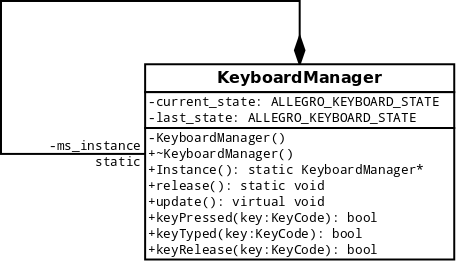
\includegraphics[scale = 0.6]{uml/KeyboardManager.png}
\end{figure}
%
%
Realiza o gerenciamento do teclado. Possui duas variáveis do tipo ALLEGRO\_KEYBOARD\_STATE. Uma para guardar o último estado e outra para guardar o estado atual do teclado, de modo a conseguir verificar se determinada tecla foi pressionada, está sendo pressionada ou foi solta. Como o tipo ALLEGRO\_KEYBOARD\_STATE sugere, uma variável desse tipo armazena o estado (pressionada ou solta) de todas as teclas do teclado no momento em que o método \textit{update()} é chamado. Há outros três métodos que verificam se determinada tecla foi pressionada, continua pressionada ou se foi solta. Os métodos recebem como parâmetro o \textit{keycode} da tecla e retornam um tipo booleano. Abaixo temos um exemplo de uso da classe KeyboardManager.
%
%
\begin{lstlisting}

  // Inicializamos os dispositivos de entrada
  KeyboardManager* keyboard = KeyboardManager::Instance();
  
  // Atualiza o estado das teclas
  keyboard->update();
	
  // Verifica se a seta direita esta pressionada
  if( keyboard->keyPressed( ALLEGRO_KEY_RIGHT ) ) {}
  
  // Verifica se a tecla ESC foi solta
  if( keyboard->keyRelease( ALLEGRO_KEY_ESCAPE ) ) {}
  
  // Verifica se a tecla SPACE foi pressionda
  if( keyboard->keyTyped( ALLEGRO_KEY_SPACE ) ) {}
	      
\end{lstlisting}
%
\subsubsection{MouseManager}
%
%
\begin{figure}[H]
    \centering
		\caption{UML detalhando a classe MouseManager.}
    \label{MouseManager}
    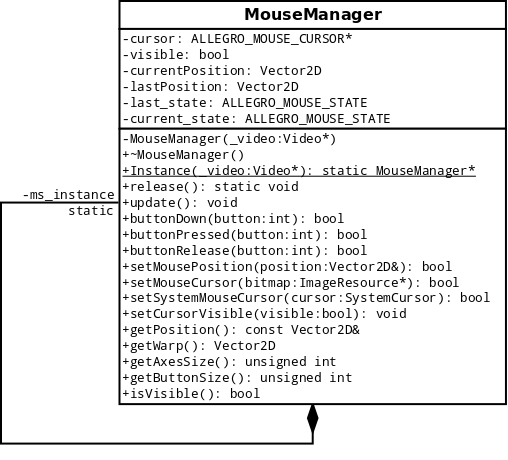
\includegraphics[scale = 0.50]{uml/MouseManager.png}
\end{figure}
%
%
Realiza o gerenciamento dos eventos gerados pelo \textit{mouse}. A classe trabalha usando lógica semelhante a KeyboardManager, só que aplicada ao mouse. Possibilita também deixar ou não visível o cursor do mouse na aplicação e alterar o estilo do cursor.
%
%
%=============================================================
\subsection{SGL Font}
%
%
É o pacote responsável pela parte textual da biblioteca. Ele carrega uma fonte no formato TTF (``True Type Font'') padrão do Windows e a utiliza para escrever um texto na tela.
%
%
%
\begin{figure}[H]
    \centering
		\caption{UML das classes FontResource e Font.}
    \label{Font}
    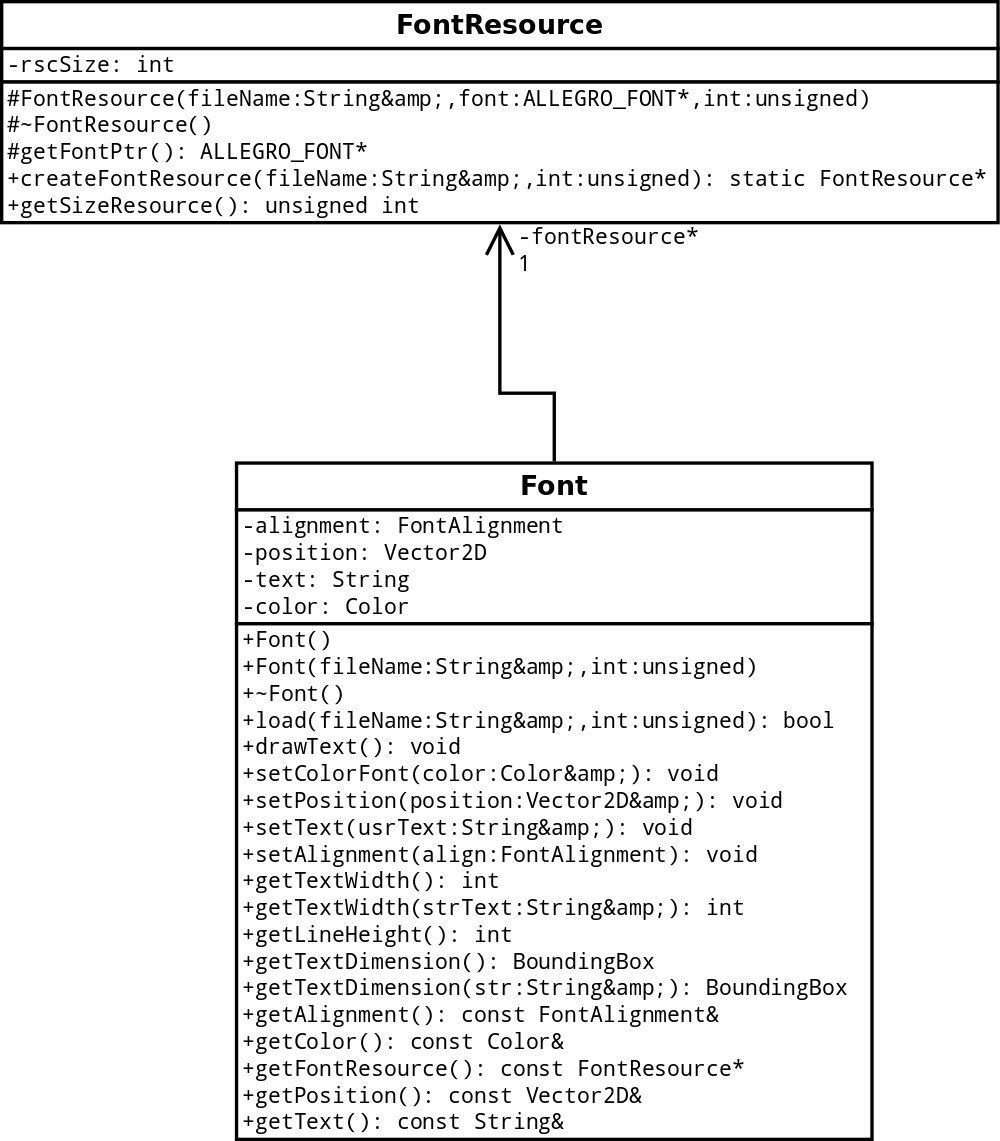
\includegraphics[scale = 0.20]{uml/Font.png}
\end{figure}
%
%
\subsubsection{FontResource}
%
%
Especialização de Resource. Ela é usada dentro do método \textit{load()} da classe Font e funciona da seguinte maneira: recebe um arquivo TTF e o tamanho da fonte desejada, e em seguida esse arquivo é adicionado a uma instância da classe ResourceManager, caso ainda não tenha sido alocado. É possível existir dois arquivos de fonte iguais mas com tamanhos diferentes em ResourceManager, isso possibilita que utilizemos fontes iguais, mas com tamanho diferentes, uma medida necessária, uma vez que a Allegro não permite que alteremos o tamanho da fonte posteriormente.
%
%
\subsubsection{Font}
%
%
Possui métodos para escrever na tela e mudar as configurações do texto, tais como cor, alinhamento e posição. O pacote utiliza também as funcionalidades das classes Vector2D, Color e BoundingBox. Com os métodos \textit{gets} temos informações sobre as configurações atuais do objeto.
\par 
A seguir temos alguns exemplos de uso da classe. Para instanciar um objeto da classe Font utilizamos seu construtor, cujo primeiro parâmetro é o \textit{path} do arquivo TTF. A barra '/' indica hierarquia de diretórios a partir da pasta do projeto. Ou seja, dentro da pasta de projeto existe uma pasta chamada Resource e o arquivo alger.ttf se encontra nela. O segundo parâmetro é o tamanho da fonte.
%
\begin{lstlisting}
  // Criamos uma font
  Font alger("Resource/alger.ttf", 30);
\end{lstlisting}
%
\par
Alterando cor, alinhamento e posição. O tipo do alinhamento pode ser RIGHT, LEFT, CENTRE ou INTEGER.
%
\begin{lstlisting}
  // Definimos a cor da fonte
  alger.setColorFont(Color ("lightskyblue"));
  // Definimos seu alinhamento
  alger.setAlignment(FontAlignment::CENTRE);
  // Definimos sua posicao
  alger.setPosition(Vector2D(200, 100));
\end{lstlisting}
%
\par 
Definimos o texto que será exibido na tela e o escrevemos no \textit{display}:
%
\begin{lstlisting}
  // Definimos o texto a ser escrito no display
  alger.setText("Fonte: Alger");
  // Desenhamos o texto
  alger.drawText();
  // Definimos um novo texto para ser escrito
  alger.setText("Tamanho: 30");
  // Ajustamos a posicao do segundo texto
  alger.setPosition(Vector2D(200, 140));
  // Desenhamos o segundo texto na display
  alger.drawText();
  // Atualizamos o display
  video.refresh();
\end{lstlisting}
%
Após a execução do código acima, temos o seguinte texto no \textit{display}.
%
%
%
\begin{figure}[H]
    \centering
		\caption{Exemplo de uso classe Font.}
    \label{ExemploFont}
    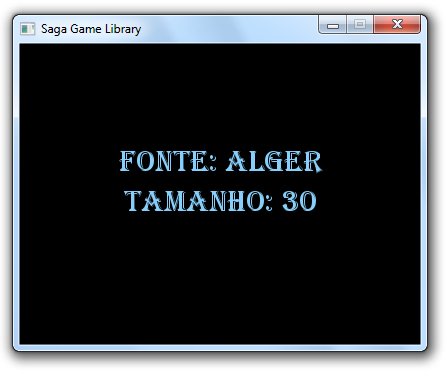
\includegraphics[scale = 0.70]{Imagens/ExemploFont.png}
\end{figure}
%
%
%
%=======================================================
\subsection{SGL Áudio}
%
%
É o pacote que realiza as funcionalidades referentes à parte sonora. É estruturado da seguinte maneira: de um lado a classe AudioResource, especialização de Resource, e da qual derivam AudioStreamResource e AudioSampleResource. Do outro lado, temos a classe abstrata Audio, da qual derivam AudioStream e AudioSample. As duas últimas relacionam-se com as respectivas especializações de AudioResource. Tal estrutura nos possibilita criar um objeto de AudioSample quando desejamos manipular um efeito sonoro, como um soco ou o barulho de uma explosão, ou um objeto de AudioStream quando precisamos usar uma trilha sonora.
\par 
AudioSample e AudioStream possuem em comum métodos para carregar, tocar, alterar ganho, balanço, velocidade e modo de repetição. Além desses, cada classe possui outros métodos com funções específicas. Entre os vários formatos de arquivos de áudio suportados, os mais usados são .wav e .ogg. Infelizmente não existe suporte ao formato MP3, por o mesmo se tratar de um formato de áudio proprietário (e também pouco usado em jogos).
\par
Exemplos:
\par 
Cria-se um objeto de  AudioSample, indicando o caminho onde o arquivo de áudio encontra-se.
%
\begin{lstlisting}
  // Criamos um sample
  AudioSample sample("Resource/audio/palmas.wav");
\end{lstlisting}
%
Altera o ganho para 80\% do valor original e a velocidade para 90\% do valor original.
%
\begin{lstlisting}
  // Ajustamos o valor do ganho
  sample.setGain(0.8);
  // Ajustamos a velocidade de execucao do sample
  sample.setSpeed(0.9);
\end{lstlisting}
%
Faz com que o arquivo continue tocando indefinidamente após chamar o método \textit{play()}.
%
\begin{lstlisting}
  // Ajustamos para reproducao em loop
  sample.setLoopingMode(AudioPlayMode::PLAY_LOOP);
\end{lstlisting}
%
Finalmente, colocamos o arquivo para ser reproduzido.
%
\begin{lstlisting}
  // Iniciamos a reproducao do sample
  sample.play();
\end{lstlisting}
%
%
Carrega um arquivo para ser reproduzido como trilha sonora e recebe parâmetros para alterar o \textit{buffer} (em \textit{bytes}) e a taxa de amostragem.
%
\begin{lstlisting}
  // Carregamos um audiostream
  AudioStream stream("Resource/audio/interface.ogg", 4, 1024);
\end{lstlisting}
%
Fazemos o arquivo tocar a partir dos 14 segundos.
%
\begin{lstlisting}
  // Definimos o tempo de inicio
  stream.setBegin(14);
  // Iniciamos a reproducao do audio stream
  stream.play();
\end{lstlisting}
%
%
%==============================================
%
\subsection{SGL Image}
%
Trata-se de um dos principais pacotes da \textit{SAGA Game Library}, contendo todas as classe referentes à manipulação de recursos de imagem. Apesar do pacote possuir um grande volume de classes, nos limitaremos às suas duas classes mais importantes: AnimatedSprite e TMXTileMap.
%
%
%
\subsubsection{TMXTileMap}
%
%
%
A grande maioria dos jogos eletrônicos 2D apresenta, além dos \textit{sprites} dos personagens e itens, uma imagem representando o cenário do jogo. Dependendo da natureza do jogo, esses cenários podem possuir grandes dimensões, o que torna custoso em termos computacionais armazenar essa imagem em memória (RAM e disco) e desenhá-la no \textit{display}. Entretanto, quando analisamos a imagem que representa o cenário, podemos verificar que o mesmo é formado por pequenas partes que se repetem com muita frequência. 

Assim, aproveitando dessa característica, com o objetivo de diminuir o consumo de memória e o desempenho na renderização e carregamento das imagens de resolução elevada, foi desenvolvida uma técnica conhecida como \textit{TileMap} \cite{Novak}, que consiste no uso de uma imagem, chamada \textit{tileset}, contendo pequenos pedaços de imagens, conhecidos como \textit{tiles}, que são as imagens que se repetem em grande quantidade no cenário do jogo. Esses \textit{tiles} são usados para criar uma imagem composta denominada \textit{tiled layer}.
%
%
\begin{figure}[H]
    \centering
		\caption{Exemplo de \textit{tileset}. Fonte: OpenGameArt}
    \label{tileset_edit}
    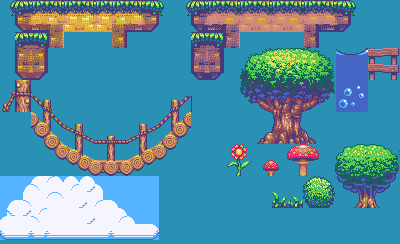
\includegraphics[scale = 1.0]{Imagens/tileset_edit.png}
\end{figure}
%
\par
O cenário final do jogo pode ser constituído de um único \textit{tiled layer} ou ser resultante da combinação de dois ou mais \textit{tiled layers}. Através da técnica de \textit{Tilemap}, torna-se possível construir inúmeros cenários, com variadas dimensões, usando como base o mesmo \textit{tilesets}, aumentando a economia de memória e não reduzindo o desempenho no carregamento de imagens.
%
%
%
\begin{figure}[H]
    \centering
		\caption{Exemplo de um cenário construído com tileset.}
    \label{cenario}
    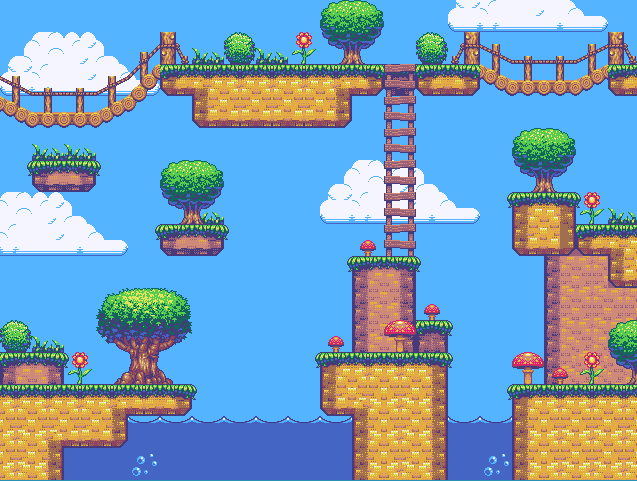
\includegraphics[scale = 0.65]{Imagens/cenario.png}
\end{figure}
%
%
%
%
\par 
A \textit{SAGA Game Library} também faz uso da técnica para criação de cenários e \textit{sprites} animados através do \textit{Tiled}. O Tiled nos fornece um arquivo XML personalizado chamado TMX, contendo todos os dados relevantes para a construção do cenário do jogo, e para ter acesso a esses dados torna-se necessário o uso de uma \textit{parser} XML, para realizar a leitura do arquivo XML. O \textit{parser} escolhido foi a TinyXML, por sua baixa curva de aprendizado e velocidade de leitura. A seguir podemos visualizar um exemplo simples de um arquivo .tmx.
%
%
\lstinputlisting{CodigoFonte/novo.tmx}
%
\par 
Como pode ser observado, o arquivo .tmx possui todos os detalhes de cada \textit{tileset} usado na construção do cenário e os dados referentes a cada \textit{layer} criado. Uma das dificuldades de implementação do suporte ao Tiled foi desenvolver as rotinas de leitura desses dados, de modo a torná-las rápidas e de fácil uso. O resultado desse trabalho foi o desenvolvimento de classes responsáveis pela leitura de cada elemento do arquivo, de forma que cada um desses dados fosse armazenados em atributos para posteriormente serem usados pelo usuário. Assim foram implementadas as classe TMXTileSet e TMXLayer entre outras. Cada uma dessas classes é responsável por realizar o \textit{parser} dos seus respectivos elementos e atributos (do arquivo .tmx). Por exemplo, a classe TMXLayer é responsável pela leitura dos elementos \textit{layer} e de seus respectivos atributos, \textit{name, width} e \textit{height} e também é responsável pela leitura, compressão (GZIP ou ZLIB) e decodificação (base64) usadas no elemento \textit{data}.
%
\par 
Quando observamos a \textit{data} do arquivo .tmx, verificamos que ela possui dois atributos: \textit{encoding} e \textit{compression}. Esses atributos nos indicam se foi usada algum tipo de codificação (base64) e se algum algoritmo de compressão (GZIP ou ZLIB foi aplicado. Para a descompressão foi utilizada a biblioteca ZLIB, que fornece métodos para se trabalhar com compressão usando GZIP e ZLIB, e para a decodificação foi usada o algoritmo desenvolvido por René Nyffenegger \footnote{http://www.adp-gmbh.ch/cpp/common/base64.html}, que fornece um modo muito prático de decodificação. Ambos os algoritmos, de compressão e descompressão funcionam da mesma maneira, é passada uma \textit{string} contendo os dados codificados/comprimidos e como retorno temos a \textit{string} decodificada/descomprimida. 

Através dessa \textit{string}, nós criamos um vetor de inteiros (através da conversão de tipos) que contem os índices de cada \textit{tile} do \textit{tileset}. Feito isso, podemos desenhá-los, fazendo com que o nosso cenário criado seja visualizado no \textit{display}. Finalmente, a classe TMXTileMap contem os métodos para carregar e manipular os dados obtidos pela leitura do arquivo tmx, também provendo rotinas de verificação de colisão entre \textit{sprites}. Esse processo de decodificação e descompressão representou um desafio, exigindo uma pesquisa sobre as bibliotecas usadas e o correto modo de usá-las.
%
%
\begin{figure}[ht]
    \centering
		\caption{Cenário construído usando o Tiled e a classe TMXTileMap.}
    \label{snapshot1}
    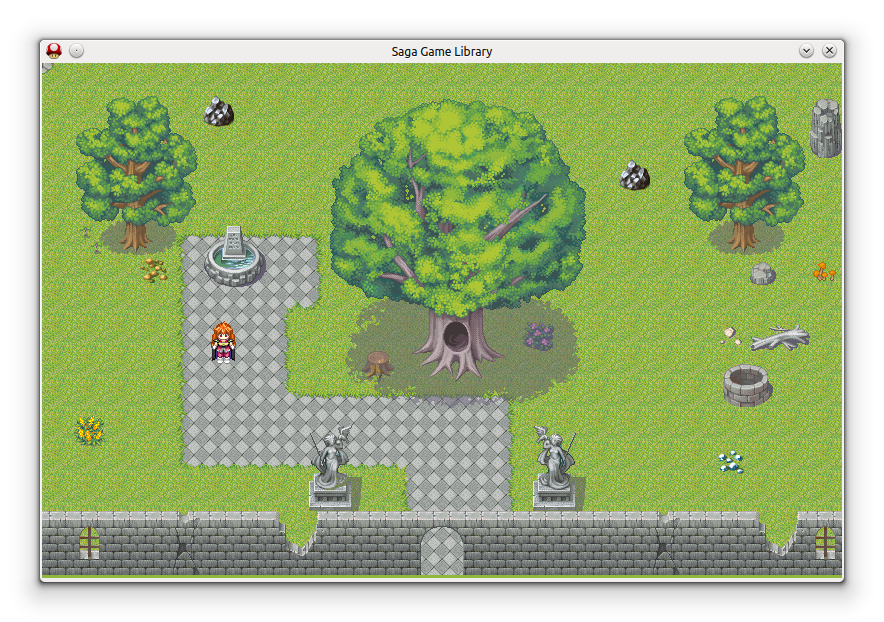
\includegraphics[scale = 0.60]{Imagens/snapshot1.png}
\end{figure}
%
\par 
Como pode-se observar, o Tiled fornece grande comodidade no projeto de cenários, uma vez que toda a tarefa se torna algo visual. Pensando nisso, também foi adaptado o uso do Tiled para criarmos \textit{sprites} animados. As classes envolvidas são as mesmas usadas para se trabalhar com os cenários (com exceção da classe TMXTileMap).
%
%
\subsubsection{AnimatedSprite}
%
%
\textit{Sprites} podem ser descritos como arquivos de imagem que suportam criação de animações e posicionamento livre na tela. De um modo geral, todas as imagens que possuem movimentação em um jogo podem ser denominadas \textit{sprites} e podem apresentar um quadro fixo ou podem ter um conjunto de animações \cite{Novatec}. Os \textit{sprites} que não possuem animação são representados pela classe StaticSprite. Esta classe recebe um objeto ImageResource e o manipula, definindo sua posição no \textit{display}, realizando a renderização e verificando se ocorreu colisão desse com outro \textit{sprite}. Quanto à classe AnimatedSprite, ela apresenta funções muito mais complexas e interessantes, as quais serão abordadas a seguir.
\par 
A classe AnimatedSprite, como o nome sugere, é usada quando se deseja ter um \textit{sprite} com suporte a animações. Essas animações são criadas através do Tiled, e carregadas posteriormente pelo método \textit{load()} da classe. Um objeto da classe AnimatedSprite é constituído de um vetor de objetos do Animation, que por sua vez possui uma coleção de objetos da classe Frame. Essas classes, como seus respectivos nomes sugerem, são responsáveis por armazenar os dados de cada animação criada para o \textit{sprite} animado.
%
%
%
\begin{figure}[H]
    \centering
		\caption{UML com detalhes das classe AnimatedSprite e suas classes auxiliares.}
    \label{AnimatedSprite}
    \includegraphics[scale = 0.40]{uml/AnimatedSprite.png}
\end{figure}
%
%
A criação das animações faz uso de um \textit{tileset} chamado \textit{spritesheet} (Figura \ref{sprite}) que contem todas as imagens referentes às animações que o \textit{sprite} pode possuir. Cada animação possui um número de \textit{frames}, que são os quadros com o desenho do personagem em uma dada posição.
%
%
%
\begin{figure}[H]
    \centering
		\caption{Exemplo de \textit{spritesheet}. Fonte: \cite{Sithjester} }
    \label{sprite}
    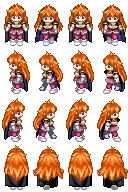
\includegraphics[scale = 1]{Imagens/sprite.png}
\end{figure}
%
%
%%
\par 
As animações são identificadas por \textit{labels} que são definidos durante a criação das animações com o Tiled e posteriormente podem ser acessadas com o método \textit{setCurrentAnimation()} da classe AnimatedSprite. O uso da AnimatedSprite proporciona grandes vantagens ao desenvolvedor ao oferecer suporte ao Tiled, tornando a criação de animações uma tarefa visual e mais atraente, fazendo uso do gerenciado de recursos ResourceManager para carregamento dos \textit{spritesheets} e possibilitando uso prático das animações. Vale ressaltar que a Allegro não possui suporte nativo à criação de \textit{sprites} animados, deixando o desenvolvedor responsável por implementar esse recurso. Felizmente, esse detalhe é contornado com o uso da AnimatedSprite, deixando o desenvolvedor livre para se focar em outras áreas mais importantes de seu projeto.
%
\par 
Para criarmos um \textit{sprite} animado usando a somente a Allegro, começamos definindo a estrutura de cada \textit{frame}.
%
\begin{lstlisting}
  /* Constantes do sprite */
  const int MAX_FRAMES  = 12;
  const int NUM_COLUNAS = 5;
  const int NUM_LINHAS  = 3;
  
  /* Definimos as propriedades do sprite */
  typedef struct Sprite
  {
      // Recebe o bitmap do sprite
      ALLEGRO_BITMAP* vetorSprites[ MAX_FRAMES ];
      // Guarda posicao dos sprites
      float pos_x, pos_y;
  } Sprite;
\end{lstlisting}
%
Em seguida criamos um \textit{sprite} que possui apenas uma animação. Essa animação funciona em \textit{loop}, ou seja, quando o último \textit{frame} da animação for desenhado, a animação volta a se repetir desde o primeiro \textit{frame}.
%
\lstinputlisting{CodigoFonte/SpriteExemplo.cpp}
%
\par 
A seguir, temos a criação de um \textit{sprite} animado usando a classe AnimatedSprite, considerando que já temos o arquivo .tmx com todas as animações prontas.
%
\lstinputlisting{CodigoFonte/ExemploAnimatedSprite.cpp}
%
Com o código acima, fica evidente a vantagem de usar a AnimatedSprite para criar \textit{sprites} animados ao invés de utilizar a Allegro separadamente.
%
%
%
\section{Testes}
%
A fase de testes consistiu simplesmente no uso das classes implementadas buscando erros de execução e \textit{bugs}. Não foi utilizada nenhuma ferramenta específica para testes de \textit{software}, devido à pouca experiência da equipe com essas ferramentas, ao tempo disponível para terminar essa versão do projeto e também à constatação das vantagens da \textit{SAGA Game Library}, não só na performance, mas também na usabilidade. Muitos dos resultados dos testes foram descritos nesse relatório, como as medições de consumo de memória e o tempo de carregamento da classe ResourceManager. 
%


